\newsection{Project Description}

Project description: The project developed an AI system, implemented as a chatbot, to reliably, transparently, and audibly assist in managing and interacting with government datasets. By combining \textbf{Retrieval-Augmented Generation (RAG)}, vectorized metadata,
and a tool-calling architecture, the system delivers grounded responses with full audit trails. Advanced AI techniques ensure ethical, accountable, and privacy-preserving outputs. The system enhances government decision-making with over
 \textbf{99\% multi-factor confidence scoring}.

\newsubsection{Datasets Used}

\begin{itemize}
    \item \href{https://www.finance.gov.au/government/procurement/statistics-australian-government-procurement-contracts-}{Australian Government Procurement Statistics}
    \begin{itemize}
        \item AusTender is the Australian Government’s procurement information system, where
        entities publish details of planned procurements, tenders, standing oQers, and awarded
        contracts in line with Commonwealth Procurement Rules.
    \end{itemize}
    \item \href{https://www.data.gov.au/data/dataset/freedom-of-information-statistics}{Freedom of Information Statistics}
    \begin{itemize}
        \item The Freedom of Information Statistics dataset contains detailed information on FOI
        activity reported by Australian Government agencies and ministers. The dataset also
        records review numbers and estimated costs, with agency-reported staQ time adjusted
        using a salary multiplier in the Excel version.
    \end{itemize}
    \item \href{https://www.kaggle.com/datasets/manishkumar21324/employee-leave-tracking-data}{Employee Leave Tracking Data (Kaggle)}
    \begin{itemize}
        \item  This dataset records employee leave details for 2024 across various departments,
        including leave type, duration, entitlements, and balances.
    \end{itemize}
\end{itemize}


\newsubsection{Data Story}

Government agencies oversee vast volumes of datasets but often struggle to extract meaningful insights efficiently. Traditional AI chatbots show potential but fail to meet the extremely high accuracy standards required in public sector decision-making, where even a 90% correct response rate may be insufficient. This gap creates challenges in trust, accurate, and accountability.

While recent advancements in AI, including large language models with advanced reasoning capabilities, promise sophisticated analysis, they also introduce risks such as hallucination, where outputs may be factually incorrect or unsupported by reliable sources. For government applications, accuracy and verifiability outweigh advanced reasoning; AI systems must provide grounded, scope-limited responses and allow human users to guide interpretation and decision-making.


\newsubsection{Our Mission}

Government agencies across Australia manage vast volumes of critical data. Despite
this, converting these resources into actionable insights remains a major challenge.
High-stakes decisions require near perfect accuracy, transparency, and accountability
standards that traditional AI often cannot meet.

\newsubsection{Current Limitations}

\begin{enumerate}
    \item Accuracy Gap – Commercial AI tools typically achieve around 90\% accuracy. For
    government decisions, this is insufficient; outcomes must meet 99\%+ reliability.
    \item Hallucination Risk – Generative AI may fabricate information, which is
    unacceptable when shaping public policy or delivering essential services.
    \item Auditability Crisis – Black-box AI outputs lack traceability, making it diQicult to
    explain or justify decisions.
    \item Integration Complexity – Departmental silos prevent seamless cross-functional
    insights.
    \item Trust Deficit – Officials cannot fully rely on AI outputs without verifiable
    evidence and clear governance.
\end{enumerate}

\clearpage
\newsubsection{System Architecture}

\begin{figure}[h]
    \centering
    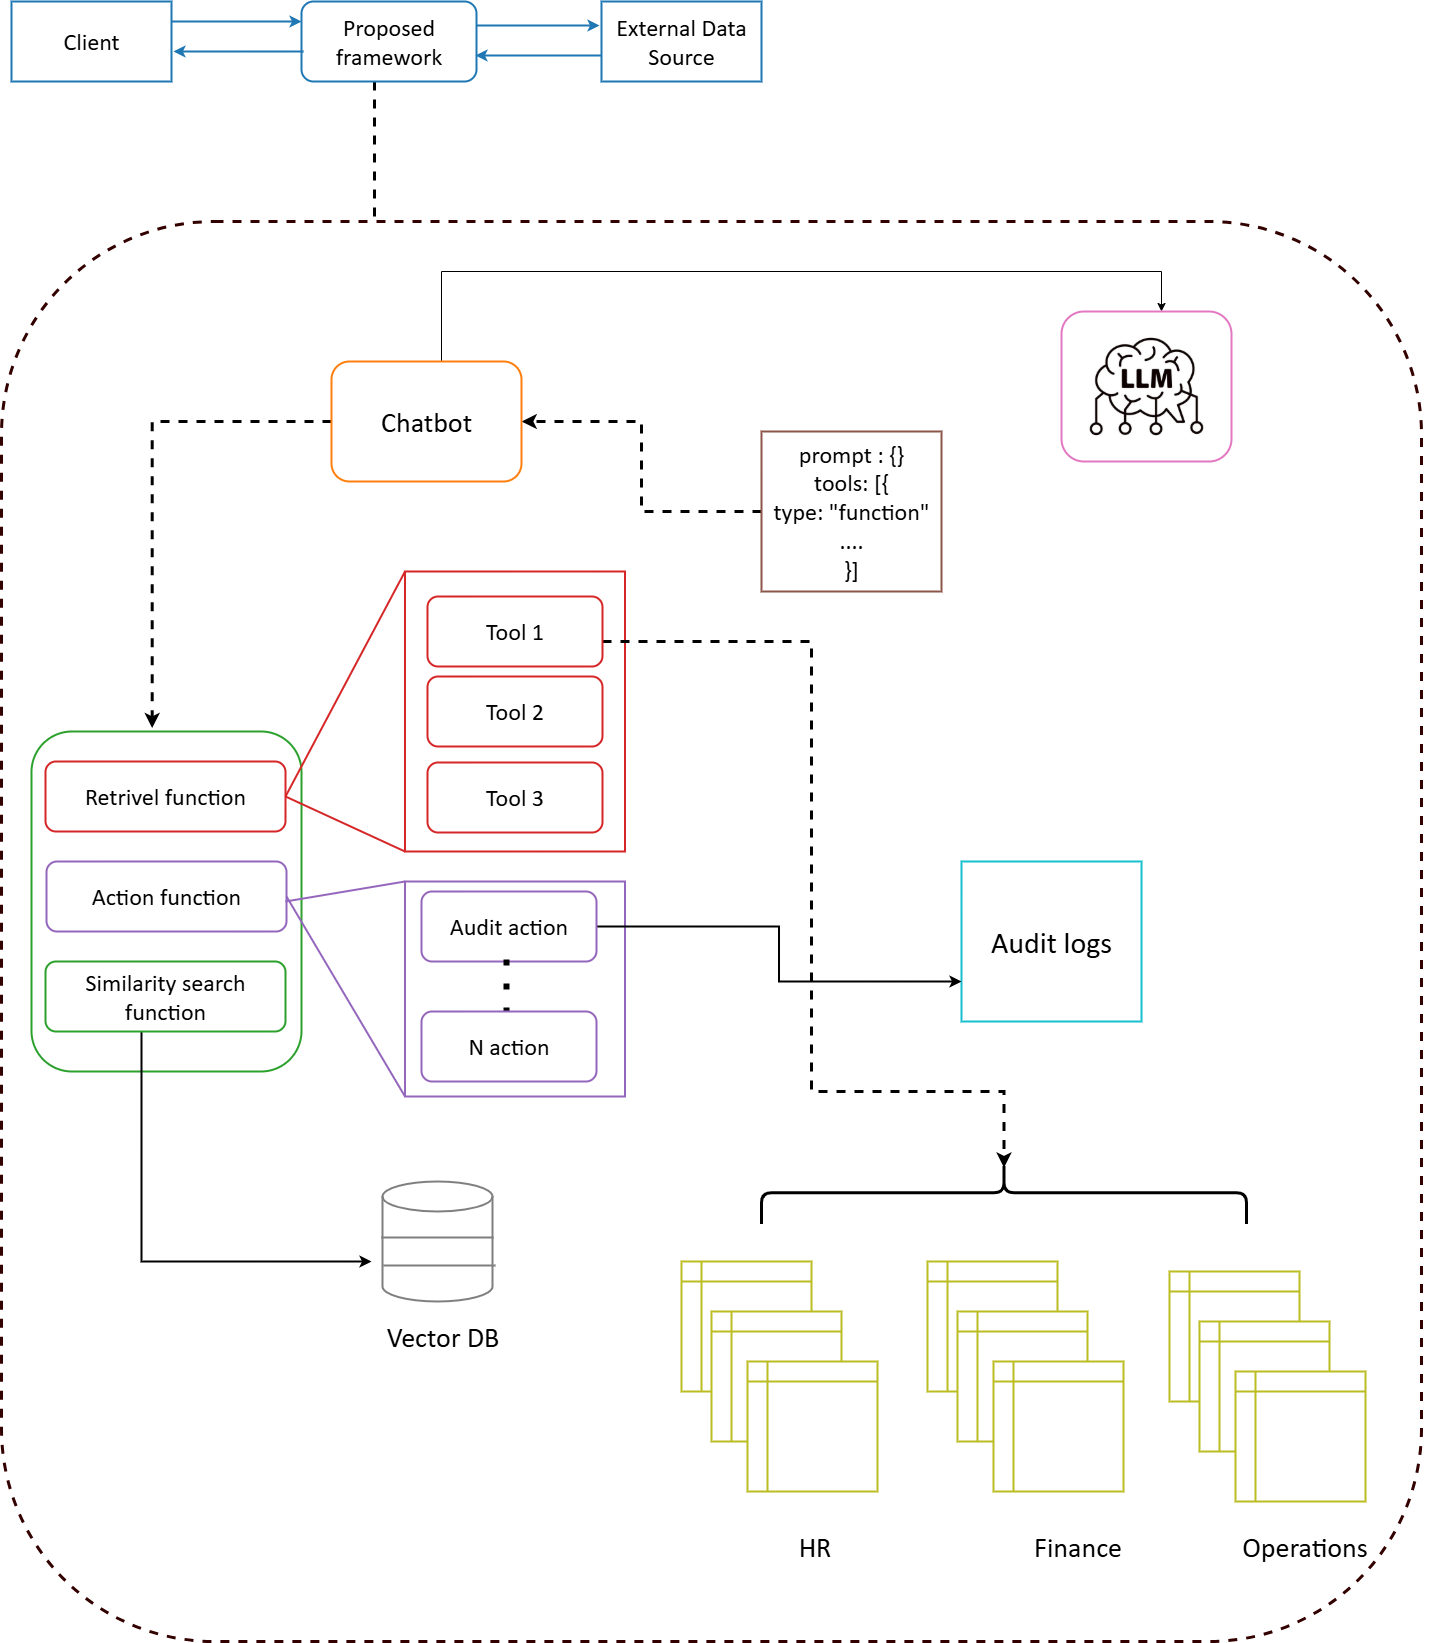
\includegraphics[width=0.85\linewidth]{img/GovHack-Architecture}
    \caption{System Architecture Diagram}
\end{figure}


\newsubsection{Our Approach}

We designed an AI system focused on \textbf{reliability, transparency, and inclusivity},
combining advanced AI techniques with governance measures:

\begin{itemize}
    \item \textbf{Retrieval-Augmented Generation (RAG):} Ensures AI responses are anchored to
    verified government sources, minimizing hallucination. 
    \item \textbf{Conversational interactions} to ensure better engagement. 
    \item \textbf{Vectorised Metadata:} Provides contextual understanding and accurate cross-
    referencing of diverse datasets. 
    \item \textbf{Tool-Calling Architecture:} Integrates multiple data sources in a modular and
    secure way, allowing scalable workflows.
    \item \textbf{Mathematical Aggregation \& Statistics:} Supports evidence-based reasoning
    and quantitative validation of AI outputs. 
    \item \textbf{Audit Logging:} Captures all prompts and responses, maintaining a complete
    history for accountability. 
    \item \textbf{Source Referencing:} Every response is linked to original datasets to ensure
    verifiability.
\end{itemize}

\newsubsection{Key Features \& Capabilities}


\begin{itemize}
    \item Multi-Factor Confidence Scoring: Evaluates the reliability of every AI output.
    \item Plain Language Summaries: Makes complex government information
    accessible to all literacy levels.
    \item Cross-Silo Interoperability: Ensures outputs can be reviewed, explained, and
    justified to meet governance standards.
\end{itemize}

\clearpage
\newsubsection{Objectives We Achieved}

\begin{figure}[h]
    \centering
    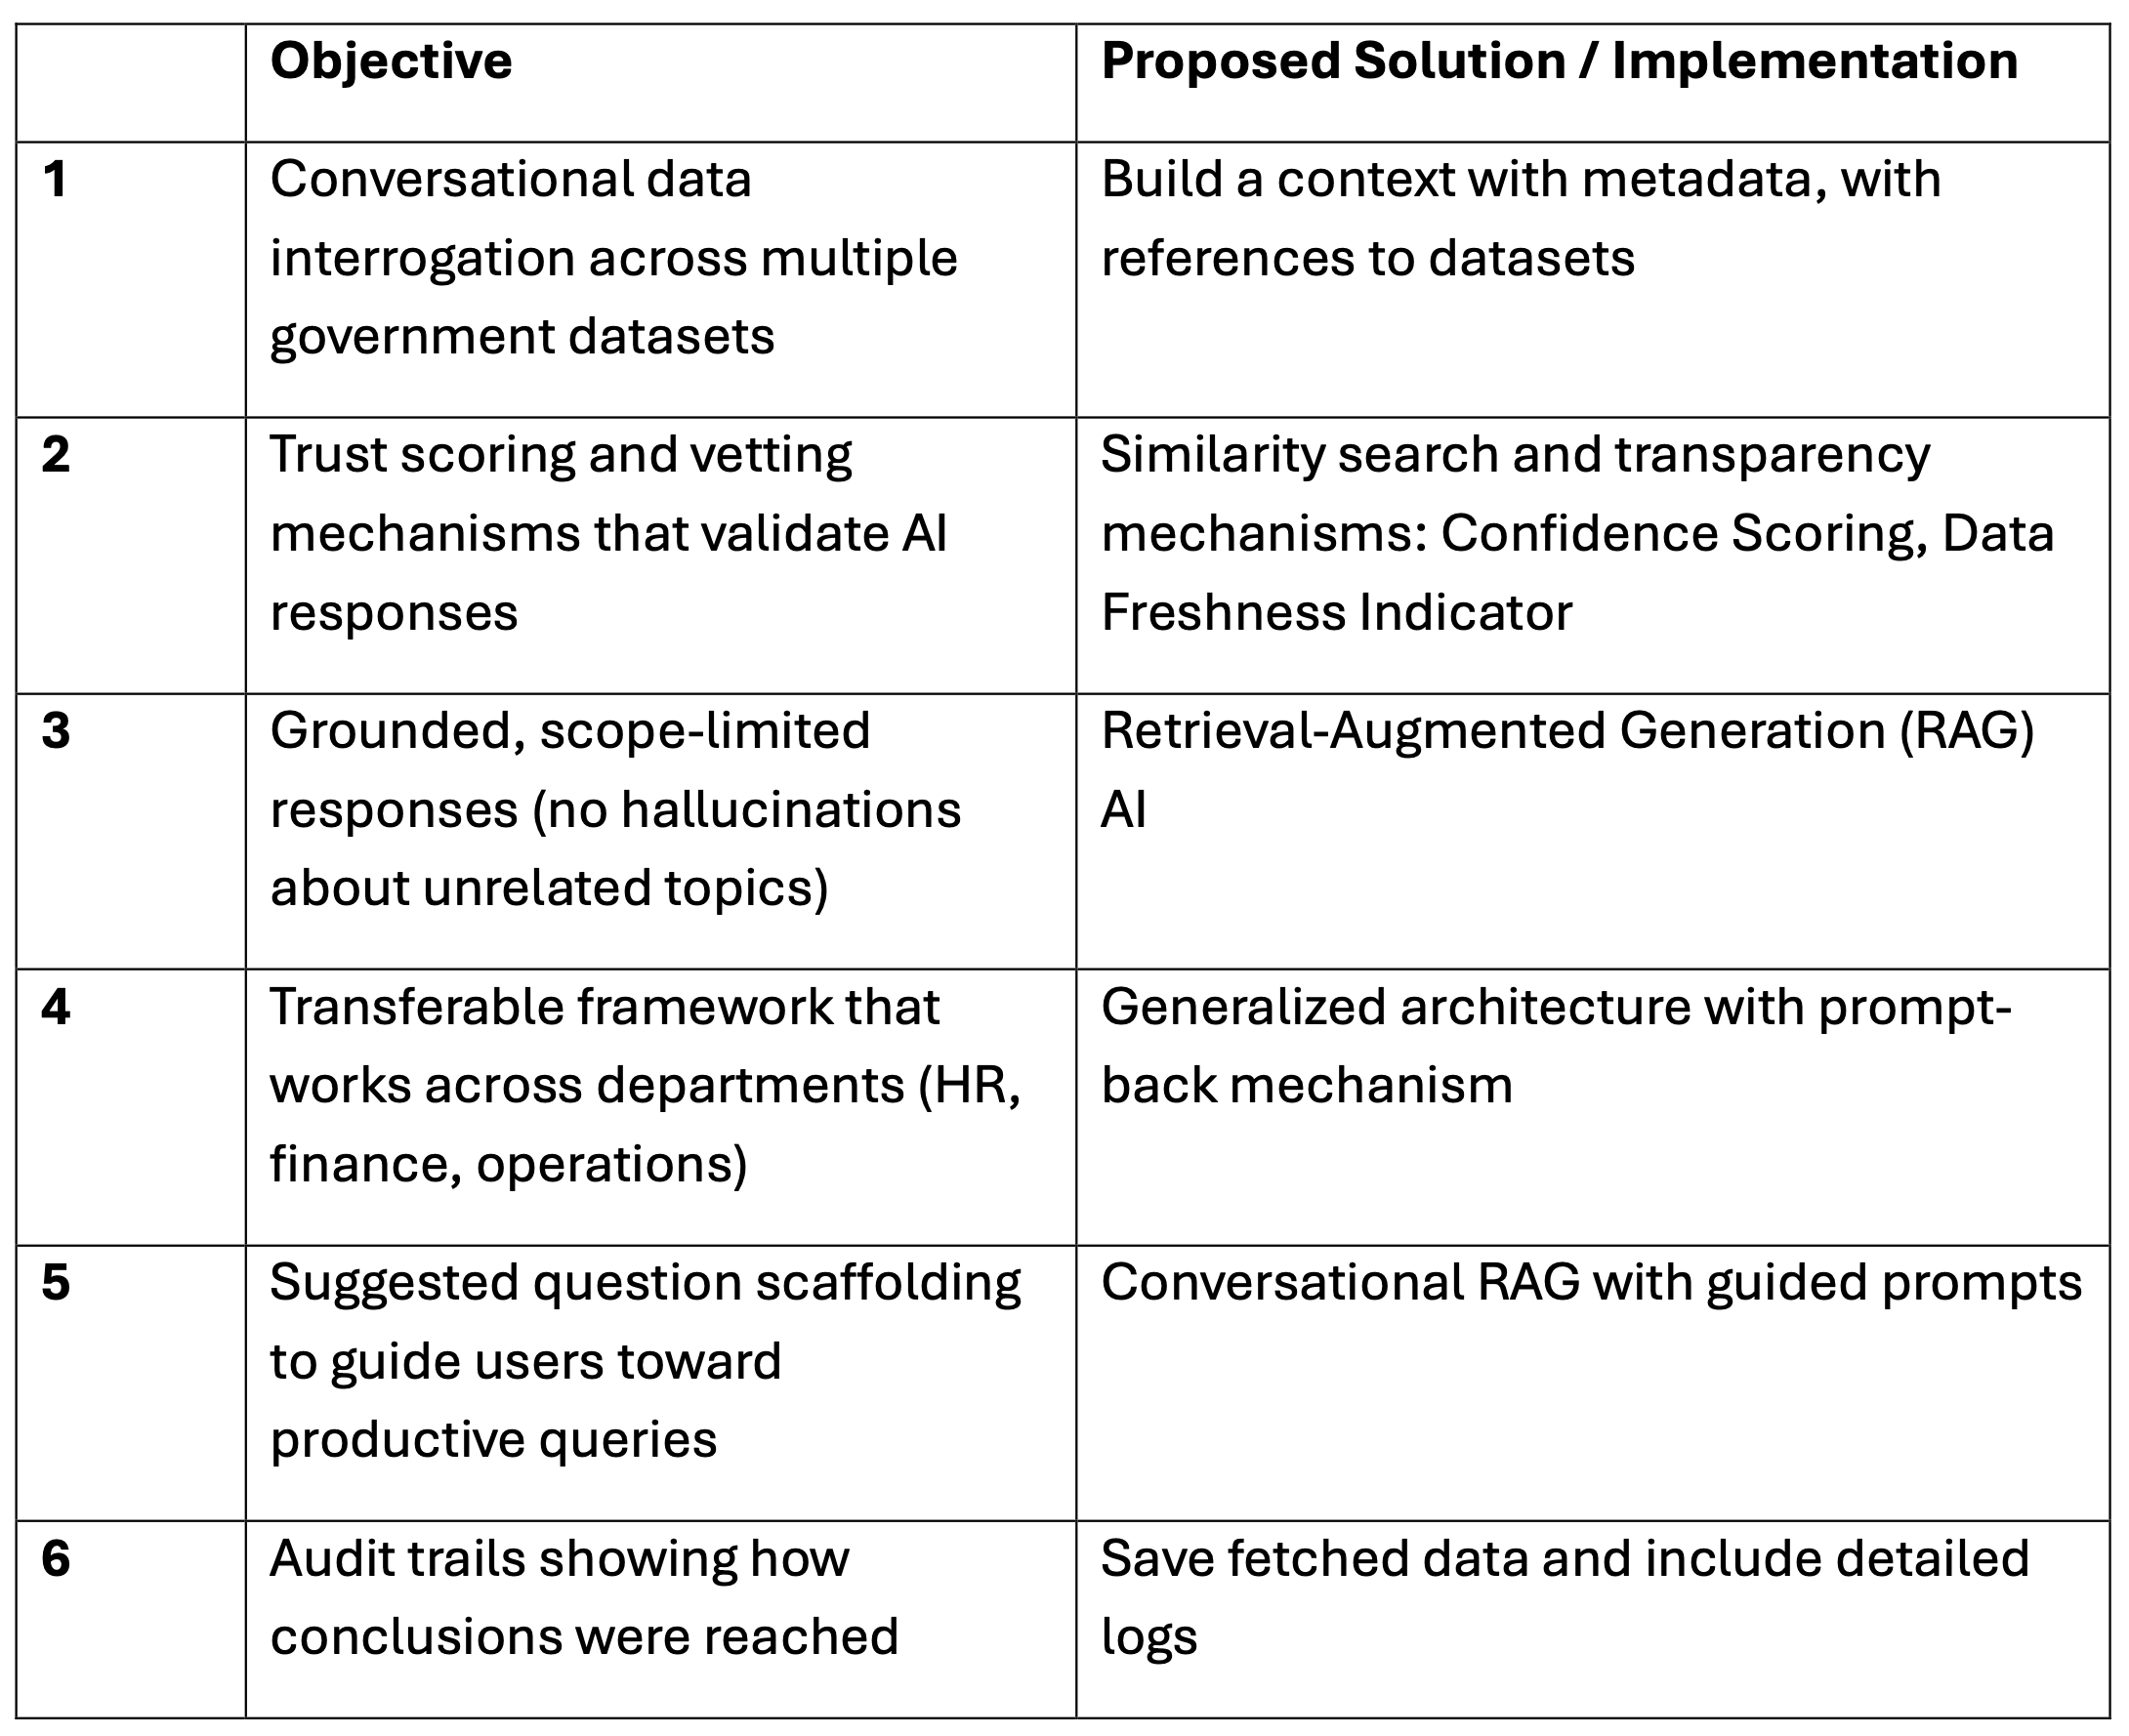
\includegraphics[width=0.75\linewidth]{img/images2}
    \caption{System Architecture Diagram}
\end{figure}


\newsubsection{Example Applications and Explanations}

\begin{enumerate}
    \item Finance:
    \begin{itemize}
        \item Use Case: Detect anomalies in vendor payments or forecast budget
        compliance.
        \item Explanation: The AI system analyzes transactional and financial datasets to flag
        unusual payment patterns, such as duplicate invoices or unexpected
        expenditure spikes. It also aggregates historical spending trends to provide
        accurate forecasts, helping finance teams make informed budgeting decisions
    \end{itemize}
    while reducing risk.
    \item Human Resources (HR):
    \begin{itemize}
        \item Use Case: Analyze leave trends and workforce patterns to support operational
        planning.
        \item Explanation: By examining HR records, timesheets, and leave applications, the
        AI identifies patterns such as high absenteeism in specific departments or
        seasonal workforce gaps. This insight helps managers plan staQing levels,
        improve team productivity, and optimize resource allocation.
    \end{itemize}
    \item Operations:
    \begin{itemize}
        \item Use Case: Identify irregularities in procurement or service delivery metrics.
        \item Explanation: The system evaluates operational data across procurement,
        logistics, and service records to spot inconsistencies, delays, or inefficiencies.
        Alerts are generated for potential issues, enabling operational managers to take
        proactive measures and maintain service quality.
    \end{itemize}
\end{enumerate}


\newsubsection{Outcomes Achieved}

Our system demonstrates how AI can be safely and e]ectively deployed in
government contexts:

\begin{itemize}
    \item Reduced Misinformation: AI outputs are grounded in verified data, reducing
    errors.
    \item Enhanced Transparency: Full audit logs and source references enable
    accountability.
    \item Improved Accessibility: Citizens and staQ can interact in natural language and
    understand outputs in plain English.
    \item Stronger Collaboration: Cross-agency integration allows unified insights and
    better-informed decision-making.
\end{itemize}

\newsubsection{Advanced AI Techniques}

To deliver reliable and accountable AI services, we leverage cutting-edge
technologies:
\begin{itemize}
    \item Retrieval-Augmented Generation (RAG): Ensures AI responses are accurate
    and grounded in trusted, authoritative data sources.
    \item Agent-Based Validation: Autonomous agents review and confirm query results
    before presenting them, maintaining high standards of accuracy and
    responsibility.
    \item Governance and Transparency Dashboards: Monitors AI performance,
    accessibility, and compliance with ethical principles, providing clear visibility for
    both government staQ and citizens.
\end{itemize}

\newsubsection{Technology Stack}

\begin{itemize}
    \item Java Runtime - 17 or above
    \item NPM latest version
    \item Homebrew
    \item NPM latest version
    \item Expo
    \item React
    \item GIT
    \item Docker
    \item Maven
    \item Spring Framework
\end{itemize}

\newsubsection{Tools \& Softwares}
\begin{itemize}
    \item Canva
    \item GenAI
    \item Excel
    \item Mermaid
    \item Prezi
\end{itemize}






\newsubsection{AI in Governance}

This section addresses the strategic considerations for implementing AI in government, specifically for our AI system that supports accurate, auditable, and trustworthy decision-making. It focuses on:

\begin{itemize}

\item Boosting Operational Efficiency

\item Improving Transparency

\item Multi Factor Confidence Scoring

\item Ensuring Ethical Use

\item Data Privacy and Security

\item Building Public Trust

\item Future Adaptations

\end{itemize}

\newsubsection{Boosting Operational Efficiency}

Government agencies must scale AI adoption according to organizational maturity, risk tolerance, and AI experience. Key steps include:

\begin{itemize}

\item Identify High-Impact Areas: Evaluate where AI can meaningfully enhance workflows, reduce administrative burden, and improve citizen services.

\item Risk and Reward Assessment: Consider risks such as data privacy or misinformation, and quantify benefits like time savings, cost efficiency, and improved social inclusion.

\item Lean Business Cases: Present concise proposals highlighting costs, benefits, and expected outcomes to secure leadership support.

\item Governance Integration: Apply a structured governance framework to ensure compliance with regulations and ethical AI practices.

\item Cross-Department Collaboration: Encourage resource and knowledge sharing to maximize efficiency and reduce duplication of effort.

\item Pilot Projects: Test AI solutions with proof-of-concept initiatives before full deployment.

\end{itemize}

\newsubsection{Improving Transparency}

Transparency is critical for public trust and accountability:

\begin{itemize}

\item Governance Dashboards: Provide real-time AI performance insights accessible to officials and citizens.

\item Decision Traceability: Log and document all AI outputs, linking responses back to original sources.

\item Accountability Assignments: Clearly define responsible stakeholders for AI decisions.

\item Practices: Adapt strategies to reflect first-of-a-kind AI solutions, ensuring expert review and integration.

\end{itemize}

\newsubsection{Ensuring Ethical Use}

Ethical AI use requires well-defined frameworks and practical measures:

\begin{itemize}

\item Alignment with AI Principles: Incorporate human-centred values, fairness, privacy, safety, and transparency.

\item Algorithmic Bias Mitigation: Use diverse datasets, perform bias audits, and ensure inclusive design practices.

\item Explainable AI: Develop AI systems that can clearly justify their outputs to decision-makers and citizens.

\item Documentation \& Reporting: Maintain detailed records of development, decisions, and performance metrics.

\item Regulatory Oversight: Establish independent monitoring bodies to ensure compliance with ethical standards.

\item Remove Personal Identification Informations: Ensure that all data used or displayed in the AI system excludes any personal identifiers to protect privacy and maintain compliance with data protection regulations.

\end{itemize}

\newsubsection{Data Privacy and Security}

Protecting sensitive government and citizen data is essential without compromising AI functionality:

\begin{itemize}

\item Secure Architecture: Implement encryption, access controls, and model protection to prevent tampering or data theft.

\item DevSecOps Integration: Include automated security testing, code audits, and ongoing security training.

\item Advanced Measures: Apply red teaming, penetration testing, and treat AI initiatives as first-of-a-kind (FOAK) to identify vulnerabilities proactively.

\item Privacy-Preserving Techniques: Leverage differential privacy, federated learning, and homomorphic encryption for safe AI analytics.

\item Data Governance: Assign roles like data stewards to oversee proper data management and compliance.

\end{itemize}

\newsubsection{Future Adaptations}

To ensure AI systems remain effective and ethical, government agencies should:

\begin{itemize}

\item Invest in R\&D: Continuously explore emerging AI techniques like multi-agent systems.

\item Pilot Emerging Technologies: Test new AI capabilities on a limited scale before wide deployment.

\item Enhance Cybersecurity: Strengthen AI-driven defense systems to protect sensitive data.

\end{itemize}

\newsubsection{Retrieval-Augmented Generation (RAG)}

\begin{itemize}

\item Data Processing: Transforms unstructured content into formats suitable for vectorized storage and efficient retrieval.

\end{itemize}

\newsubsection{Semantic Matching}

Recognizes contextually similar terms to deliver more accurate and meaningful responses.

\newsubsection{AI Tool Calling}

Tool calling (function calling) enables AI models to interact with external APIs or systems, extending their capabilities. Tools are mainly used for information retrieval (e.g., RAG, querying databases, fetching news/weather) and for taking actions. While models can request tool calls with input arguments, the client application executes the calls and returns results, ensuring security.

\begin{figure}[h]
    \centering
    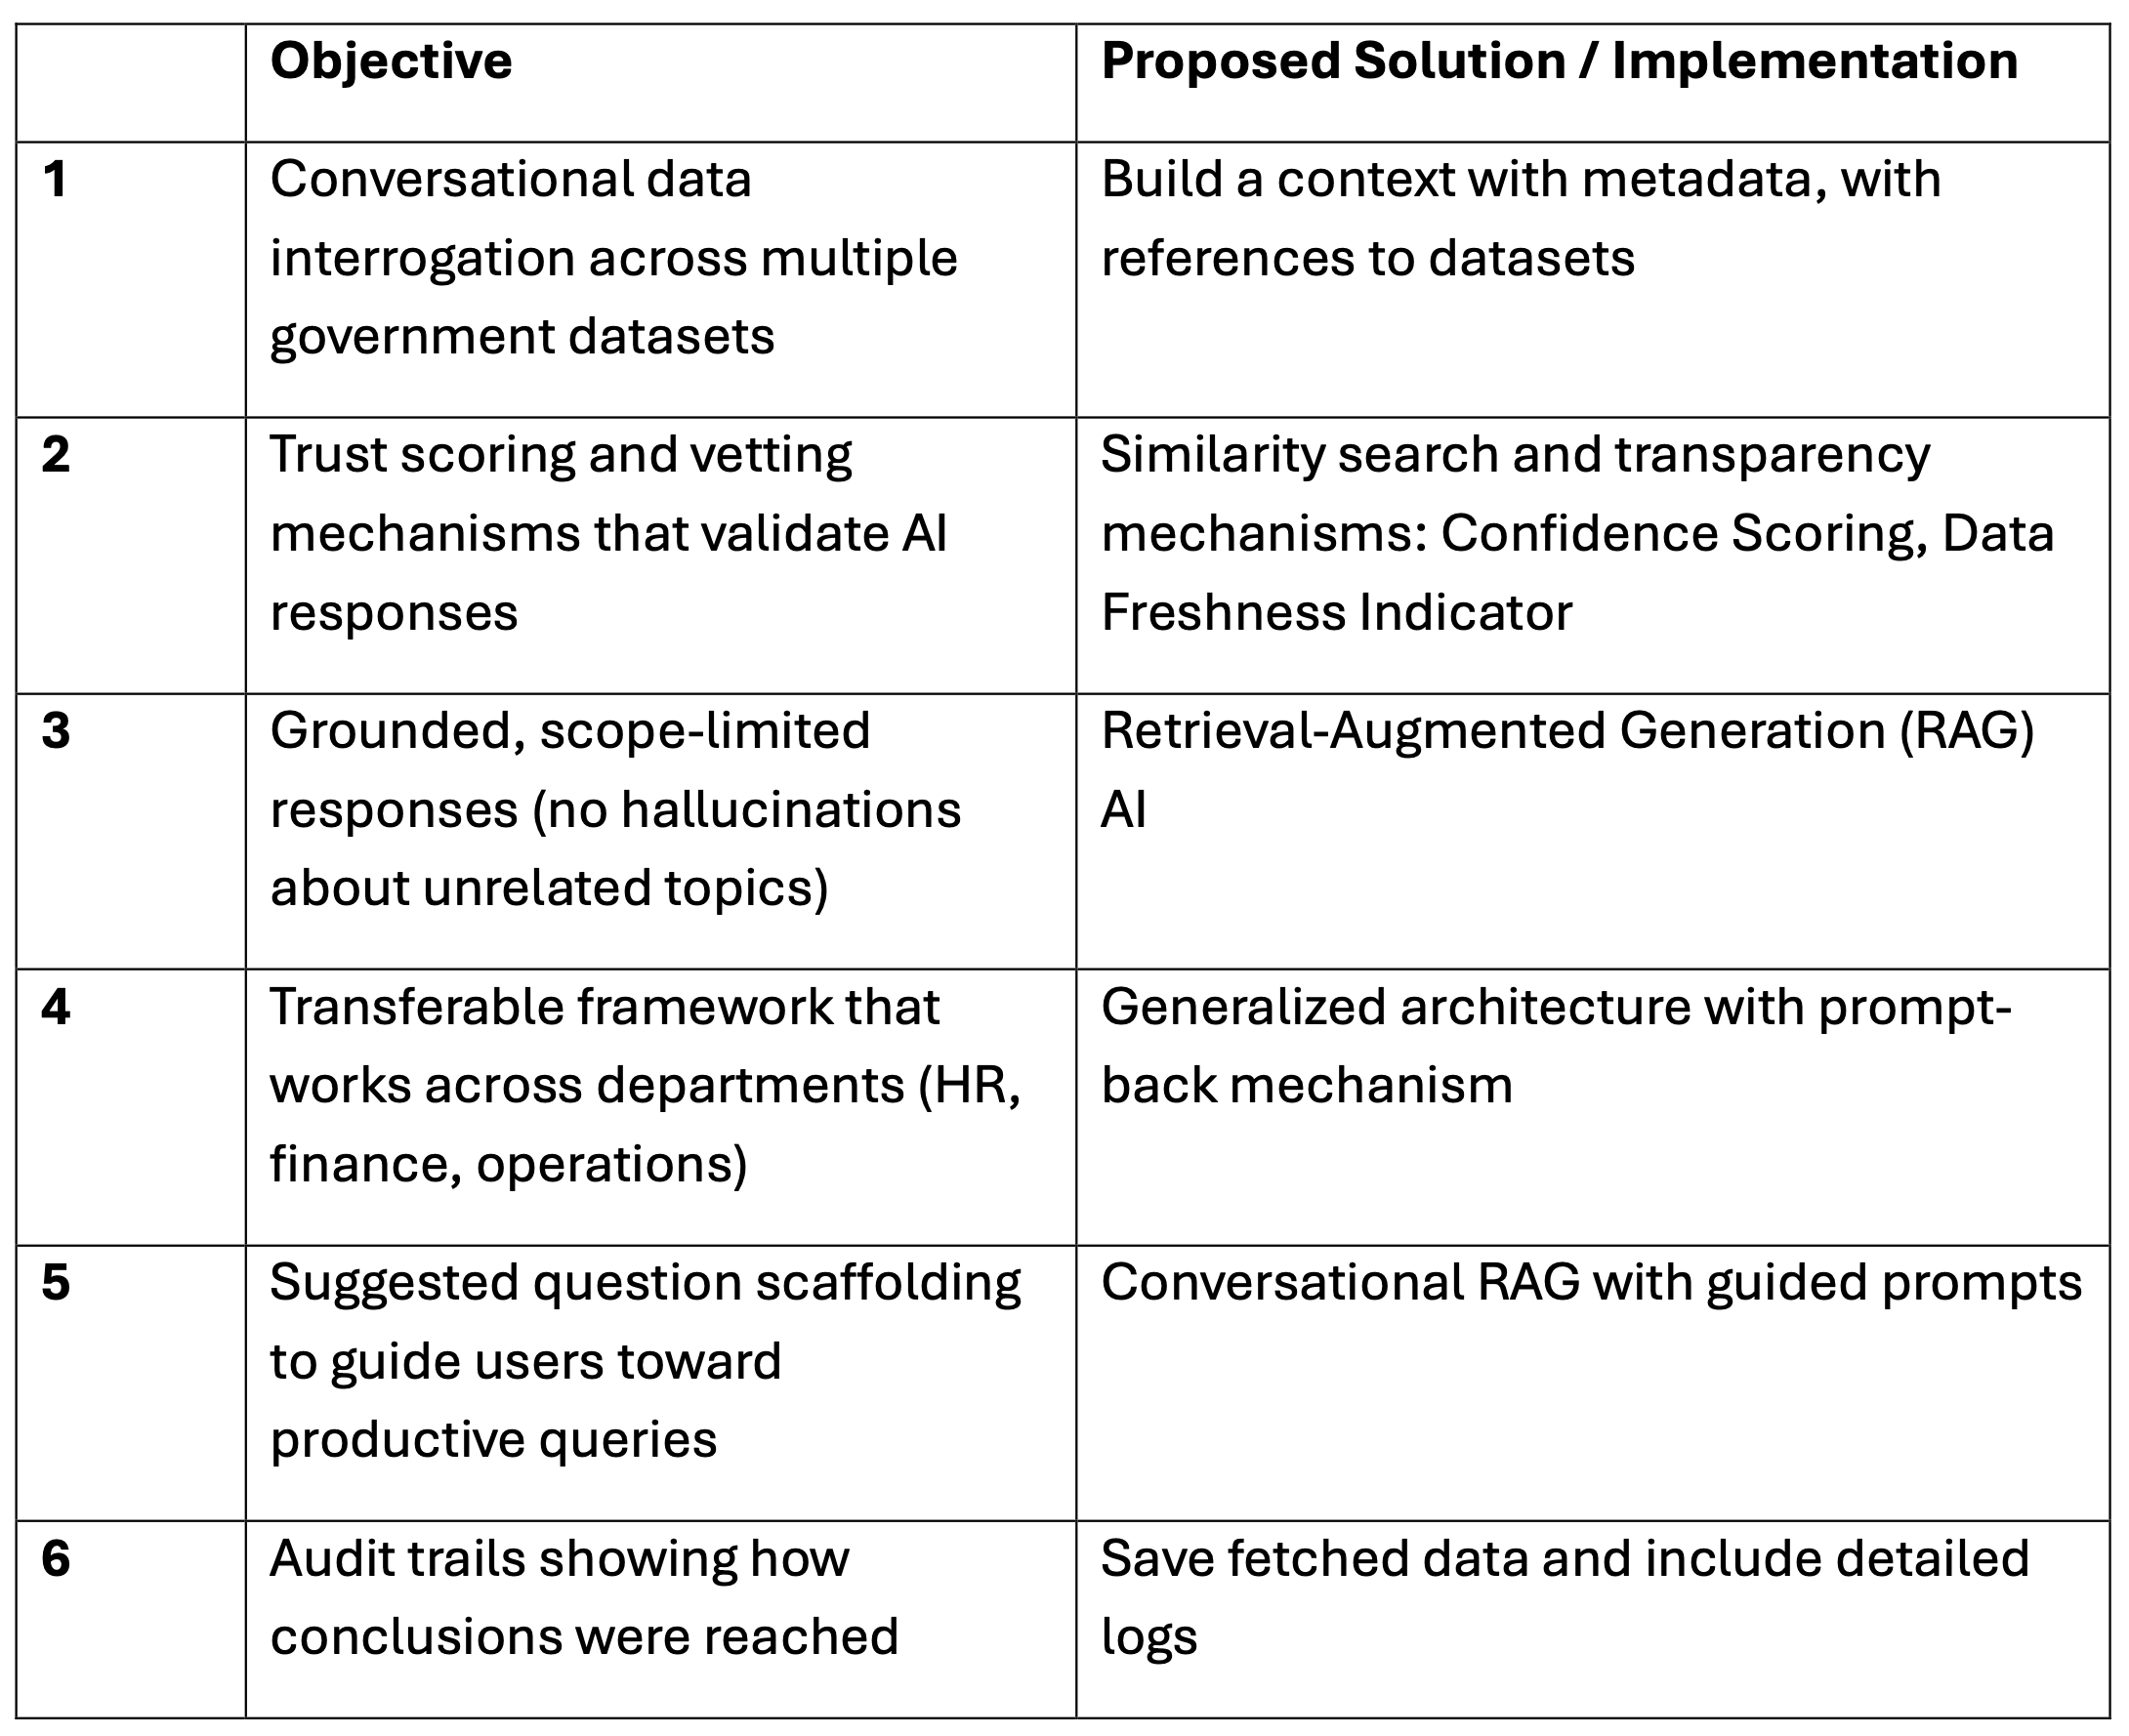
\includegraphics[width=0.85\linewidth]{img/images2}
    \caption{System Architecture Diagram}
\end{figure}

\begin{enumerate}

\item Define the tool in the chat request with a name, description, and input schema.

\item If the model decides to use the tool, it outputs the tool name and input parameters.

\item The application identifies and executes the tool with those parameters.

\item The result is processed by the application.

\item The application returns the result to the model.

\item The model generates the final response using the result as added context.

\end{enumerate}

Spring. (n.d.). \textit{Spring AI: Tools API reference}. Spring. Retrieved August 31, 2025, from \url{https://docs.spring.io/spring-ai/reference/api/tools.html}

\newsubsection{Vector Database Utilization}

\begin{itemize}

\item Scalable Access: Handles growing datasets efficiently without compromising retrieval speed.

\item Contextual Awareness: Leverages semantic understanding to provide precise and relevant information.

\end{itemize}

\newsubsection{Governance and Compliance}

\begin{itemize}

\item Alignment with AI Principles: Ensures operations adhere to standards of fairness, transparency, and accountability.

\item Performance Monitoring: Tracks metrics such as accuracy, accessibility, and fairness through a dedicated governance dashboard.

\end{itemize}








